\documentclass{standalone}
\usepackage{tikz}
\usetikzlibrary{patterns, positioning}
\usepackage[sfdefault]{ClearSans} %% option 'sfdefault' activates Clear Sans as the default text font
\usepackage[T1]{fontenc}

\begin{document}
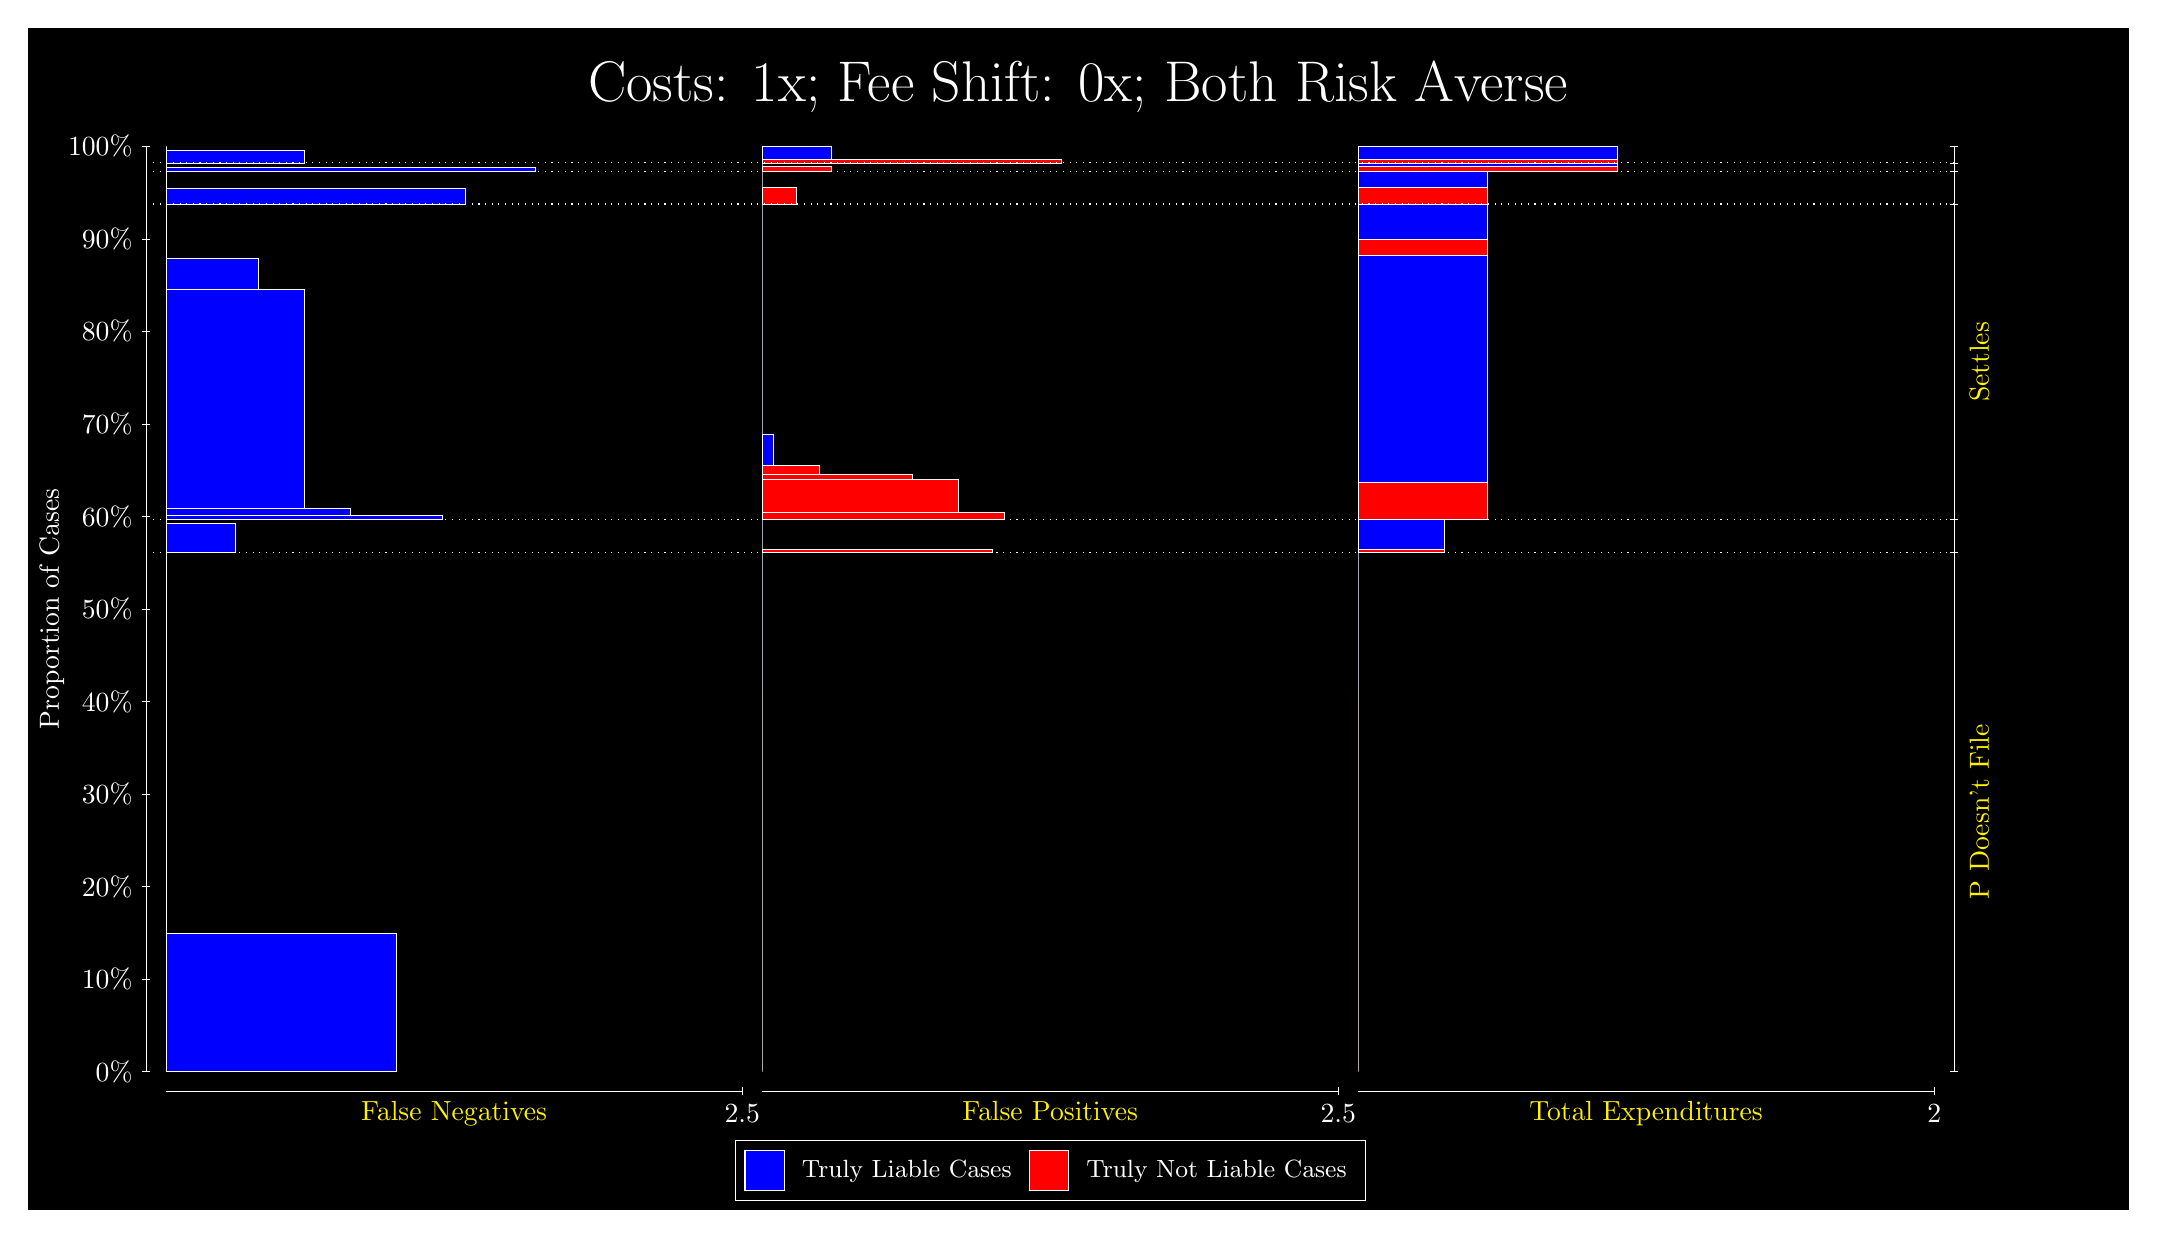
\begin{tikzpicture}
\draw[fill=black] (0,0) rectangle (26.667,15);
\draw[text=white] (0,13.5) rectangle (26.667,15) node[midway] {\huge Costs: 1x; Fee Shift: 0x; Both Risk Averse};
\draw[white, very thin] (1.5,1.75) -- (1.5,13.5);
\node[rotate=90, text=white, anchor=center] at (0.3, 7.625) {Proportion of Cases};
\draw[white, very thin] (1.45,1.75) -- (1.55,1.75);
\node[text=white, anchor=east] at (1.45, 1.75) {0\%};
\draw[white, very thin] (1.45,2.925) -- (1.55,2.925);
\node[text=white, anchor=east] at (1.45, 2.925) {10\%};
\draw[white, very thin] (1.45,4.1) -- (1.55,4.1);
\node[text=white, anchor=east] at (1.45, 4.1) {20\%};
\draw[white, very thin] (1.45,5.275) -- (1.55,5.275);
\node[text=white, anchor=east] at (1.45, 5.275) {30\%};
\draw[white, very thin] (1.45,6.45) -- (1.55,6.45);
\node[text=white, anchor=east] at (1.45, 6.45) {40\%};
\draw[white, very thin] (1.45,7.625) -- (1.55,7.625);
\node[text=white, anchor=east] at (1.45, 7.625) {50\%};
\draw[white, very thin] (1.45,8.8) -- (1.55,8.8);
\node[text=white, anchor=east] at (1.45, 8.8) {60\%};
\draw[white, very thin] (1.45,9.975) -- (1.55,9.975);
\node[text=white, anchor=east] at (1.45, 9.975) {70\%};
\draw[white, very thin] (1.45,11.15) -- (1.55,11.15);
\node[text=white, anchor=east] at (1.45, 11.15) {80\%};
\draw[white, very thin] (1.45,12.325) -- (1.55,12.325);
\node[text=white, anchor=east] at (1.45, 12.325) {90\%};
\draw[white, very thin] (1.45,13.5) -- (1.55,13.5);
\node[text=white, anchor=east] at (1.45, 13.5) {100\%};

\draw[white, very thin] (24.457,1.75) -- (24.457,13.5);
\draw[white, very thin] (24.407,1.75) -- (24.507,1.75);
\node[anchor=west] at (24.407, 1.75) {};
\draw[white, very thin] (24.407,8.341) -- (24.507,8.341);
\node[anchor=west] at (24.407, 8.341) {};
\draw[white, very thin] (24.407,8.7578) -- (24.507,8.7578);
\node[anchor=west] at (24.407, 8.7578) {};
\draw[white, very thin] (24.407,12.768) -- (24.507,12.768);
\node[anchor=west] at (24.407, 12.768) {};
\draw[white, very thin] (24.407,13.182) -- (24.507,13.182);
\node[anchor=west] at (24.407, 13.182) {};
\draw[white, very thin] (24.407,13.291) -- (24.507,13.291);
\node[anchor=west] at (24.407, 13.291) {};
\draw[white, very thin] (24.407,13.5) -- (24.507,13.5);
\node[anchor=west] at (24.407, 13.5) {};

\draw[white, very thin, fill=blue] (1.75,1.75) rectangle (4.6775,3.5104);
\draw[white, very thin, fill=red] (1.75,3.5104) rectangle (1.75,8.341);
\draw[white, very thin, fill=blue] (1.75,8.341) rectangle (2.6283,8.7188);
\draw[white, very thin, fill=red] (1.75,8.7188) rectangle (1.75,8.7578);
\draw[white, very thin, fill=blue] (1.75,8.7578) rectangle (5.2631,8.8086);
\draw[white, very thin, fill=blue] (1.75,8.8086) rectangle (4.092,8.8985);
\draw[white, very thin, fill=blue] (1.75,8.8985) rectangle (3.5065,11.688);
\draw[white, very thin, fill=blue] (1.75,11.688) rectangle (2.921,12.081);
\draw[white, very thin, fill=red] (1.75,12.081) rectangle (1.75,12.768);
\draw[white, very thin, fill=blue] (1.75,12.768) rectangle (5.5558,12.973);
\draw[white, very thin, fill=red] (1.75,12.973) rectangle (1.75,13.182);
\draw[white, very thin, fill=blue] (1.75,13.182) rectangle (6.4341,13.231);
\draw[white, very thin, fill=red] (1.75,13.231) rectangle (1.75,13.291);
\draw[white, very thin, fill=blue] (1.75,13.291) rectangle (3.5065,13.451);
\draw[white, very thin, fill=red] (1.75,13.451) rectangle (1.75,13.5);
\draw[white, very thin, fill=red] (9.3189,1.75) rectangle (9.3189,6.5806);
\draw[white, very thin, fill=blue] (9.3189,6.5806) rectangle (9.3189,8.341);
\draw[white, very thin, fill=red] (9.3189,8.341) rectangle (12.246,8.38);
\draw[white, very thin, fill=blue] (9.3189,8.38) rectangle (9.3189,8.7578);
\draw[white, very thin, fill=red] (9.3189,8.7578) rectangle (12.393,8.8503);
\draw[white, very thin, fill=red] (9.3189,8.8503) rectangle (11.807,9.2715);
\draw[white, very thin, fill=red] (9.3189,9.2715) rectangle (11.222,9.33);
\draw[white, very thin, fill=red] (9.3189,9.33) rectangle (10.051,9.4451);
\draw[white, very thin, fill=blue] (9.3189,9.4451) rectangle (9.4652,9.8378);
\draw[white, very thin, fill=blue] (9.3189,9.8378) rectangle (9.3189,12.768);
\draw[white, very thin, fill=red] (9.3189,12.768) rectangle (9.758,12.977);
\draw[white, very thin, fill=blue] (9.3189,12.977) rectangle (9.3189,13.182);
\draw[white, very thin, fill=red] (9.3189,13.182) rectangle (10.197,13.242);
\draw[white, very thin, fill=blue] (9.3189,13.242) rectangle (9.3189,13.291);
\draw[white, very thin, fill=red] (9.3189,13.291) rectangle (13.125,13.34);
\draw[white, very thin, fill=blue] (9.3189,13.34) rectangle (10.197,13.5);
\draw[white, very thin, fill=red] (16.888,1.75) rectangle (16.888,6.5806);
\draw[white, very thin, fill=blue] (16.888,6.5806) rectangle (16.888,8.341);
\draw[white, very thin, fill=red] (16.888,8.341) rectangle (17.986,8.38);
\draw[white, very thin, fill=blue] (16.888,8.38) rectangle (17.986,8.7578);
\draw[white, very thin, fill=red] (16.888,8.7578) rectangle (18.534,9.2375);
\draw[white, very thin, fill=blue] (16.888,9.2375) rectangle (18.534,12.117);
\draw[white, very thin, fill=red] (16.888,12.117) rectangle (18.534,12.325);
\draw[white, very thin, fill=blue] (16.888,12.325) rectangle (18.534,12.768);
\draw[white, very thin, fill=red] (16.888,12.768) rectangle (18.534,12.977);
\draw[white, very thin, fill=blue] (16.888,12.977) rectangle (18.534,13.182);
\draw[white, very thin, fill=red] (16.888,13.182) rectangle (20.181,13.242);
\draw[white, very thin, fill=blue] (16.888,13.242) rectangle (20.181,13.291);
\draw[white, very thin, fill=red] (16.888,13.291) rectangle (20.181,13.34);
\draw[white, very thin, fill=blue] (16.888,13.34) rectangle (20.181,13.5);
\draw[white, dotted] (1.5,8.341) -- (24.457,8.341);
\draw[white, dotted] (1.5,8.7578) -- (24.457,8.7578);
\draw[white, dotted] (1.5,12.768) -- (24.457,12.768);
\draw[white, dotted] (1.5,13.182) -- (24.457,13.182);
\draw[white, dotted] (1.5,13.291) -- (24.457,13.291);
\draw[white, very thin] (1.75,1.5) -- (9.0689,1.5);
\node[text=yellow, anchor=north] at (5.4094, 1.5) {False Negatives};
\draw[white, very thin] (9.0689,1.45) -- (9.0689,1.55);
\node[text=white, anchor=north] at (9.0689, 1.45) {2.5};

\draw[white, very thin] (9.3189,1.5) -- (16.638,1.5);
\node[text=yellow, anchor=north] at (12.978, 1.5) {False Positives};
\draw[white, very thin] (16.638,1.45) -- (16.638,1.55);
\node[text=white, anchor=north] at (16.638, 1.45) {2.5};

\draw[white, very thin] (16.888,1.5) -- (24.207,1.5);
\node[text=yellow, anchor=north] at (20.547, 1.5) {Total Expenditures};
\draw[white, very thin] (24.207,1.45) -- (24.207,1.55);
\node[text=white, anchor=north] at (24.207, 1.45) {2};

\node[text=yellow, centered, rotate=90] at (24.777, 5.0455) {P Doesn't File};

\node[text=yellow, centered, rotate=90] at (24.777, 10.763) {Settles};




\draw (12.978300999999998,1.5) node[draw=none] (baseCoordinate) {};
\begin{scope}[align=center]
        \matrix[scale=0.5, draw=white, below=0.5cm of baseCoordinate, nodes={draw}, column sep=0.1cm]{
            \node[rectangle, draw, minimum width=0.5cm, minimum height=0.5cm, fill=blue] {}; &
            \node[draw=none, font=\small, text=white] (B) {Truly Liable Cases}; &
            \node[rectangle, draw, minimum width=0.5cm, minimum height=0.5cm, fill=red] {}; &
            \node[draw=none, font=\small, text=white] (B) {Truly Not Liable Cases}; \\
            };
\end{scope}

\end{tikzpicture}
\end{document}